% Fixed-position renderer for the Level 1 DFD.
% Keep all visible content synchronized with level-1.mmd; adjust coordinates only.
\documentclass{article}
\usepackage[paperwidth=16cm,paperheight=19cm,margin=0cm]{geometry}
\usepackage{tikz}
\usetikzlibrary{arrows.meta,calc}
\pagestyle{empty}
\setlength{\parindent}{0pt}

\definecolor{processfill}{HTML}{E0E7FF}
\definecolor{processstroke}{HTML}{6366F1}
\definecolor{entityfill}{HTML}{F3F4F6}
\definecolor{entitystroke}{HTML}{4B5563}
\definecolor{groupfill}{HTML}{FFFDE7}
\definecolor{groupstroke}{HTML}{E2DFA4}
\definecolor{flowstroke}{HTML}{8A8A80}

\tikzset{
  process/.style={
    circle,
    draw=processstroke,
    fill=processfill,
    line width=0.8pt,
    minimum size=2.45cm,
    text width=2.05cm,
    align=center,
    inner sep=1pt,
    font=\sffamily\scriptsize
  },
  entity/.style={
    rectangle,
    draw=entitystroke,
    fill=entityfill,
    line width=0.7pt,
    minimum width=3.15cm,
    minimum height=0.65cm,
    align=center,
    inner sep=2pt,
    font=\sffamily\scriptsize
  },
  flow/.style={
    -{Stealth[length=1.8mm,width=1.2mm]},
    draw=flowstroke,
    line width=0.6pt,
    rounded corners=2pt
  },
  flowlabel/.style={
    fill=white,
    fill opacity=0.88,
    text opacity=1,
    inner sep=1.2pt,
    align=center,
    font=\sffamily\tiny
  },
  grouptitle/.style={font=\sffamily\scriptsize}
}

\begin{document}
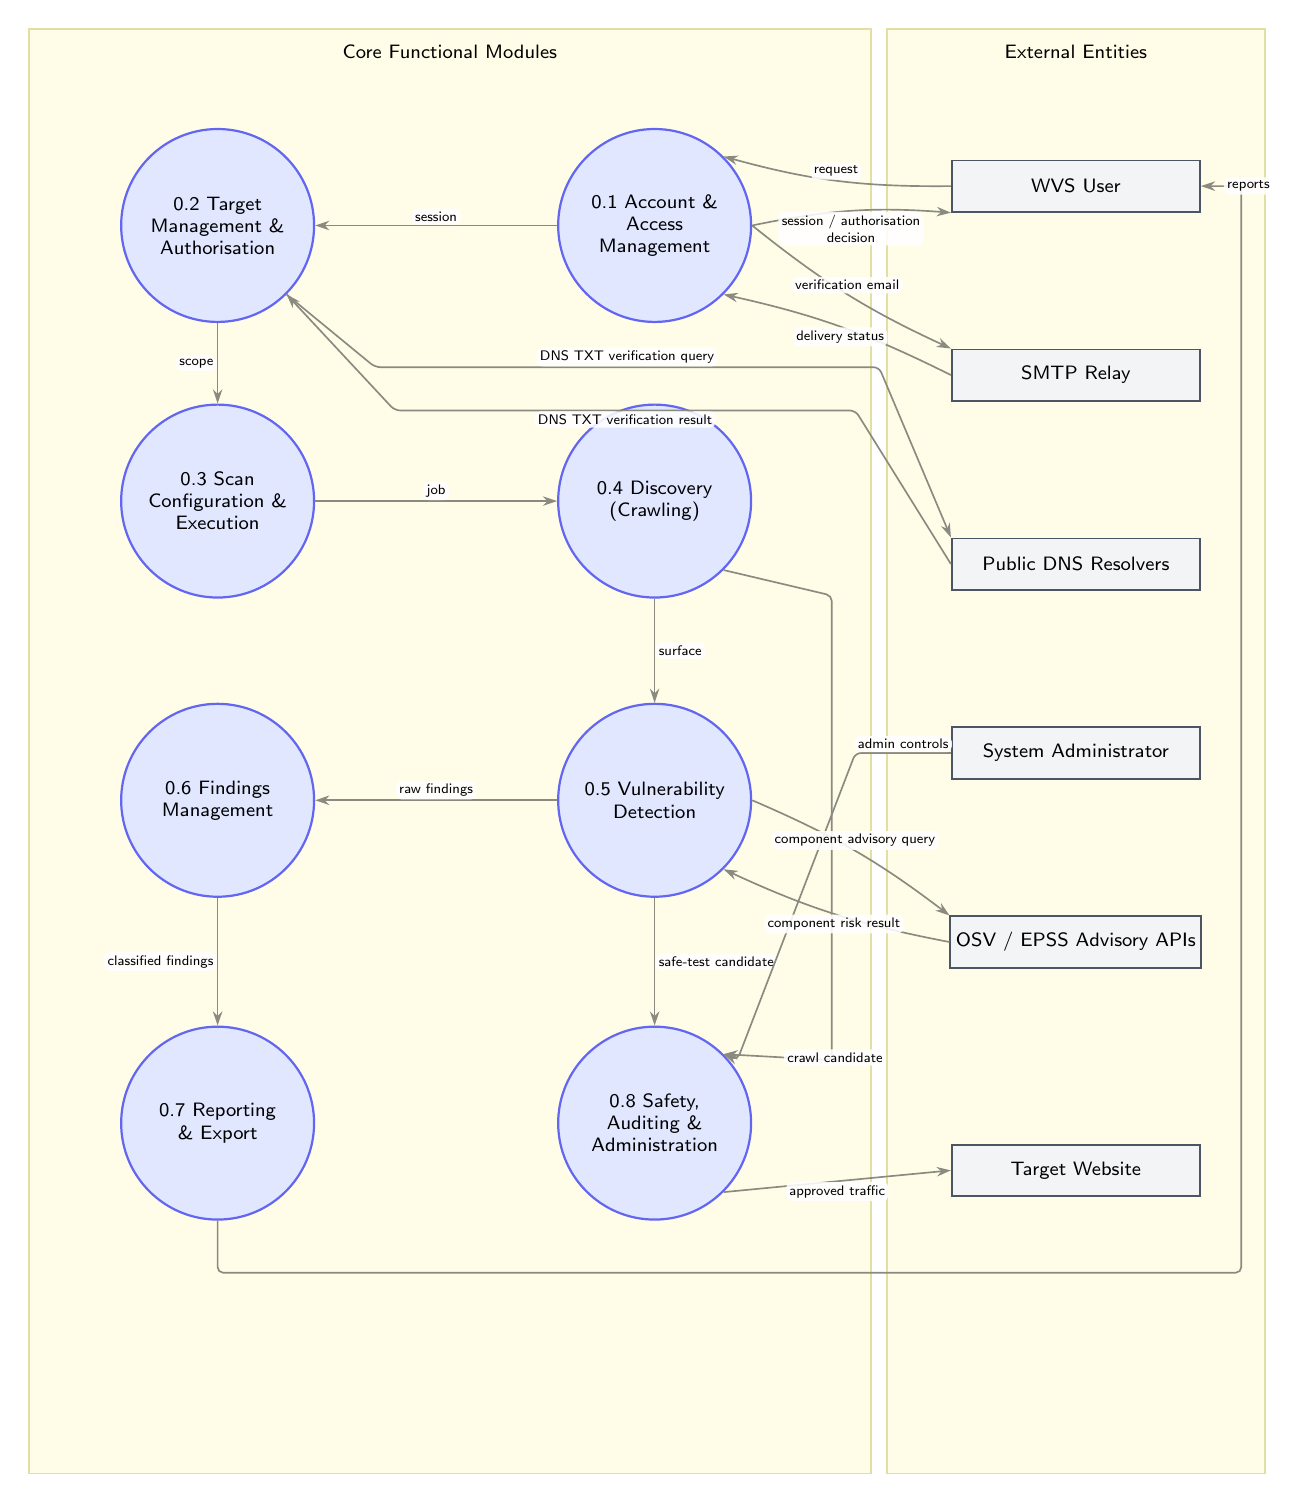
\begin{tikzpicture}[x=1cm,y=1cm]
  \path[fill=groupfill,draw=groupstroke,line width=0.7pt]
    (0.15,0.2) rectangle (10.85,18.55);
  \path[fill=groupfill,draw=groupstroke,line width=0.7pt]
    (11.05,0.2) rectangle (15.85,18.55);
  \node[grouptitle] at (5.5,18.25) {Core Functional Modules};
  \node[grouptitle] at (13.45,18.25) {External Entities};

  \node[process] (p02) at (2.55,16.05) {0.2 Target\\Management \&\\Authorisation};
  \node[process] (p01) at (8.10,16.05) {0.1 Account \&\\Access\\Management};
  \node[process] (p03) at (2.55,12.55) {0.3 Scan\\Configuration \&\\Execution};
  \node[process] (p04) at (8.10,12.55) {0.4 Discovery\\(Crawling)};
  \node[process] (p06) at (2.55,8.75) {0.6 Findings\\Management};
  \node[process] (p05) at (8.10,8.75) {0.5 Vulnerability\\Detection};
  \node[process] (p07) at (2.55,4.65) {0.7 Reporting\\\& Export};
  \node[process] (p08) at (8.10,4.65) {0.8 Safety,\\Auditing \&\\Administration};

  \node[entity] (user) at (13.45,16.55) {WVS User};
  \node[entity] (smtp) at (13.45,14.15) {SMTP Relay};
  \node[entity] (dns) at (13.45,11.75) {Public DNS Resolvers};
  \node[entity] (admin) at (13.45,9.35) {System Administrator};
  \node[entity] (osv) at (13.45,6.95) {OSV / EPSS Advisory APIs};
  \node[entity] (target) at (13.45,4.05) {Target Website};

  % Sequential main pipeline.
  \draw[flow] (p01.west) -- node[flowlabel,above] {session} (p02.east);
  \draw[flow] (p02.south) -- node[flowlabel,left] {scope} (p03.north);
  \draw[flow] (p03.east) -- node[flowlabel,above] {job} (p04.west);
  \draw[flow] (p04.south) -- node[flowlabel,right] {surface} (p05.north);
  \draw[flow] (p05.west) -- node[flowlabel,above] {raw findings} (p06.east);
  \draw[flow] (p06.south) -- node[flowlabel,left] {classified findings} (p07.north);

  % User interactions.
  \draw[flow] (user.west) to[bend left=8]
    node[flowlabel,above] {request} (p01.north east);
  \draw[flow] (p01.east) to[bend left=8]
    node[flowlabel,below] {session / authorisation\\decision} (user.south west);
  \draw[flow]
    (p07.south) -- (2.55,2.75) -- (15.55,2.75) -- (15.55,16.55)
    -- node[flowlabel,right,pos=0.45] {reports} (user.east);

  % Scope Guard and safety routing.
  \draw[flow]
    (p04.south east) -- (10.35,11.35) -- (10.35,5.45)
    -- node[flowlabel,right,pos=0.45] {crawl candidate} (p08.north east);
  \draw[flow] (p05.south) -- node[flowlabel,right] {safe-test candidate} (p08.north);
  \draw[flow]
    (admin.west) -- node[flowlabel,above] {admin controls} (10.65,9.35)
    -- (9.15,5.45) -- (p08.north east);
  \draw[flow] (p08.south east) -- node[flowlabel,below] {approved traffic} (target.west);

  % Third-party interactions.
  \draw[flow]
    (p02.south east) -- (4.55,14.25) -- node[flowlabel,above]
    {DNS TXT verification query} (10.95,14.25) -- (dns.north west);
  \draw[flow]
    (dns.west) -- (10.65,13.70) -- node[flowlabel,below]
    {DNS TXT verification result} (4.80,13.70) -- (p02.south east);

  \draw[flow] (p01.east) to[bend right=7]
    node[flowlabel,above] {verification email} (smtp.north west);
  \draw[flow] (smtp.west) to[bend right=7]
    node[flowlabel,below] {delivery status} (p01.south east);

  \draw[flow] (p05.east) to[bend left=7]
    node[flowlabel,above] {component advisory query} (osv.north west);
  \draw[flow] (osv.west) to[bend left=7]
    node[flowlabel,below] {component risk result} (p05.south east);
\end{tikzpicture}
\end{document}
